\documentclass[paper=a4, fontsize=11pt]{scrartcl} % A4 paper and 11pt font size
\usepackage{./../usfassignment}
\settitle{Assignment 5}
\setauthor{Wanzhang Sheng}
\setcourse{CS675: Automata Theory}

\begin{document}

\maketitle % Print the title

% -----------------------------------------------------------------------------
% PROBLEM 1
% -----------------------------------------------------------------------------
\section{}

\begin{fancyquotes}
  For each of the following languages, give both a context-free
  grammar and a push-down automata.
\end{fancyquotes}

\begin{enumerate}
\item
  \begin{fancyquotes}
    (8 points) $\{a^nb^{3n} : n>0\}$
  \end{fancyquotes}

  $$S\rightarrow aSbbb \mid \epsilon$$

  \begin{figure}[H]
    \centering
    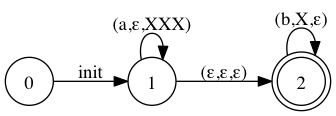
\includegraphics[scale=.7]{5-1.gv.png}
    \caption{$\{a^nb^{3n} : n>0\}$}
  \end{figure}

\item
  \begin{fancyquotes}
    (8 points) $\{a^nx : n\geq 0, x \in (a+b)^*, |x| = n \}$
  \end{fancyquotes}

  $$S\rightarrow aSa \mid aSb \mid \epsilon$$

  \begin{figure}[H]
    \centering
    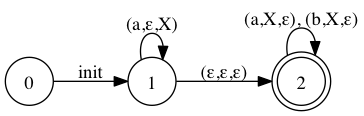
\includegraphics[scale=.7]{5-1.gv.2.png}
    \caption{$\{a^nx : n\geq 0, x \in (a+b)^*, |x| = n \}$}
  \end{figure}

\item
  \begin{fancyquotes}
    (8 points) $L =$ all strings over $\{a,b\}$ that do not contain
    the substring $bba$
  \end{fancyquotes}

  $$S\rightarrow AB$$
  $$A\rightarrow aA \mid baA \mid \epsilon$$
  $$B\rightarrow bB \mid \epsilon$$

  \begin{figure}[H]
    \centering
    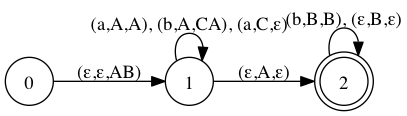
\includegraphics[scale=.7]{5-1.gv.3.png}
    \caption{$L =$ all strings over $\{a,b\}$ that do not contain the
      substring $bba$}
  \end{figure}

\item
  \begin{fancyquotes}
    (8 points) $L =$ Valid prefix operations over the alphabet 1, 2,
    3, -, /.
  \end{fancyquotes}

  $$S\rightarrow OSS \mid ONN \mid N$$
  $$O\rightarrow - \mid /$$
  $$N\rightarrow 1 \mid 2 \mid 3$$

  \begin{figure}[H]
    \centering
    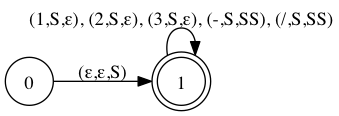
\includegraphics[scale=.7]{5-1.gv.4.png}
    \caption{$L =$ Valid prefix operations over the alphabet 1, 2, 3, -, /.}
  \end{figure}

\end{enumerate}

\pagebreak

% -----------------------------------------------------------------------------
% PROBLEM 2
% -----------------------------------------------------------------------------
\section{}

\begin{fancyquotes}
  Give a Regular Expression equivalent to each of the following
  CFGs. Think carefully about the language described by the CFG, and
  create an equivalent regular expression.
\end{fancyquotes}

\begin{enumerate}
\item
  \begin{fancyquotes}
    (3 points) $S \rightarrow ABA$, $A \rightarrow aA$,
    $A \rightarrow \epsilon$, $B \rightarrow bb$
  \end{fancyquotes}

  $a^*bba^*$
\item
  \begin{fancyquotes}
    (3 points) $S \rightarrow AB$, $A \rightarrow aAa \mid bAb \mid a
    \mid b$, $B \rightarrow aB \mid bB \mid \epsilon$
  \end{fancyquotes}

  $(a+b)^*$
\item
  \begin{fancyquotes}
    (3 points) $S \rightarrow AA$, $A \rightarrow AAA$, $A \rightarrow a$
  \end{fancyquotes}

  $aa(aa)^*$
\end{enumerate}

\pagebreak

% -----------------------------------------------------------------------------
% PROBLEM 3
% -----------------------------------------------------------------------------
\section{}

\begin{fancyquotes}
  (8 points) Give both a CFG and a PDA for the language $L$ All
  strings over $\{0,1\}$ that are not of the form $0^n1^n$. $L =
  \overline{\{0^n1^n : n > 0\}}$. Thus, $001, 100, 1001, 0110 \in L$,
  while $01, 0011, 000111 \not\in L$.
\end{fancyquotes}

CFG:
$$S\rightarrow \epsilon \mid 1A \mid NE \mid ZN \mid ZN0A$$
$$A\rightarrow 1A \mid 0A \mid \epsilon$$
$$E\rightarrow 1A \mid 0A \mid 0 \mid 1$$
$$Z\rightarrow 0Z \mid 0$$
$$N\rightarrow 0N1 \mid 01$$

\begin{figure}[hp]
  \centering
  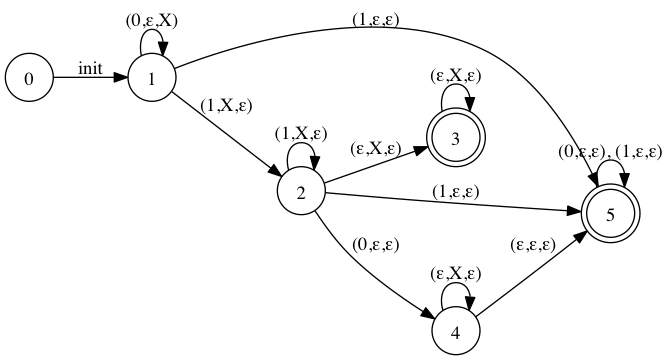
\includegraphics[width=\textwidth]{5-3.gv.png}
  \caption{$L = \overline{\{0^n1^n : n > 0\}}$}
\end{figure}

\end{document}
